\section{Traversability}

\subsection{Eulerian Graphs}

\subsubsection*{Seven Bridges of Königsberg Problem}
\begin{center}
    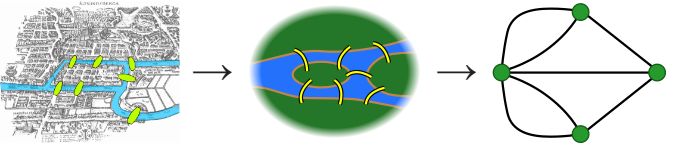
\includegraphics[width=\textwidth]{assets/6.1-bridges.png}
\end{center}
Can you go for a walk, crossing each bridge exactly once? No

\subsubsection*{Eulerian Circuits and Trails Definition}
\begin{itemize}
    \item A \bld{Eulerian Circuit} is a circuit containing every edge of graph $G$.
    \item A \bld{Eulerian Trail} is an open trail containing every edge of graph $G$.
    \item A \bld{Eulerian Graph} is a graph that contains an \itl{Eulerian Circuit}
\end{itemize}

\subsubsection*{Even Degree and Eulerian Circuits Theorem}
A nontrivial, connected graph is Eulerian if and only if \itl{every} vertex has \itl{even} degree.

\subsubsection*{Even Degree and Eulerian Trails Corollary}
A connected graph $G$ contains an Eulerian Trail, if and only if exactly 2 vertices of $G$ have odd degree.

\subsection{Hamiltonian Graphs}

\subsubsection*{Hamiltonian Cycles and Paths Definition}
\begin{itemize}
    \item A \bld{Hamiltonian Cycle} is a cycle containing every vertex of graph $G$.
    \item A \bld{Hamiltonian Path} is a path containing every vertex of graph $G$.
    \item A \bld{Hamiltonian Graph} is a graph that contains an \itl{Hamiltonian Cycle}.
\end{itemize}

\subsubsection*{Degree Sum and Hamiltonian Graphs Theorem}
Let $G$ have order $n \geq 3$. If $\deg u + \deg v \geq n$ for all pairs of nonadjacent vertices $u,v \in V(G)$, then $G$ is Hamiltonian. Note that this is only a \itl{one way} statement.

\subsubsection*{Degree Sum and Hamiltonian Graphs Corollary}
Let $G$ have order $n \geq 3$. If $\deg v \geq \frac{n}{2}$ for all $v \in V(G)$, then $G$ is Hamiltonian. Note that this is only a \itl{one way} statement.